%%% Local Variables:
%%% mode: latex
%%% TeX-master: "../main.tex"
%%% End:

\documentclass[../main.tex]{subfiles}

\begin{document}

\subsection{Introduction} Functional programming is a programming paradigm in
which programs are structured as a composition of pure functions
\autocite{Hughes1989WhyMatters}

Pure functions, by contrast to function constructs of programming languages,
refer to the mathematical concept of a function. In mathematics "a function \textit{f}
from A to B, where A and B are non-empty sets, is a rule that associates with
each element of A (the domain) a unique element of B (the codomain)"
\autocite{NicholsonTheMathematics}.

\begin{figure}[ht]
  \centering 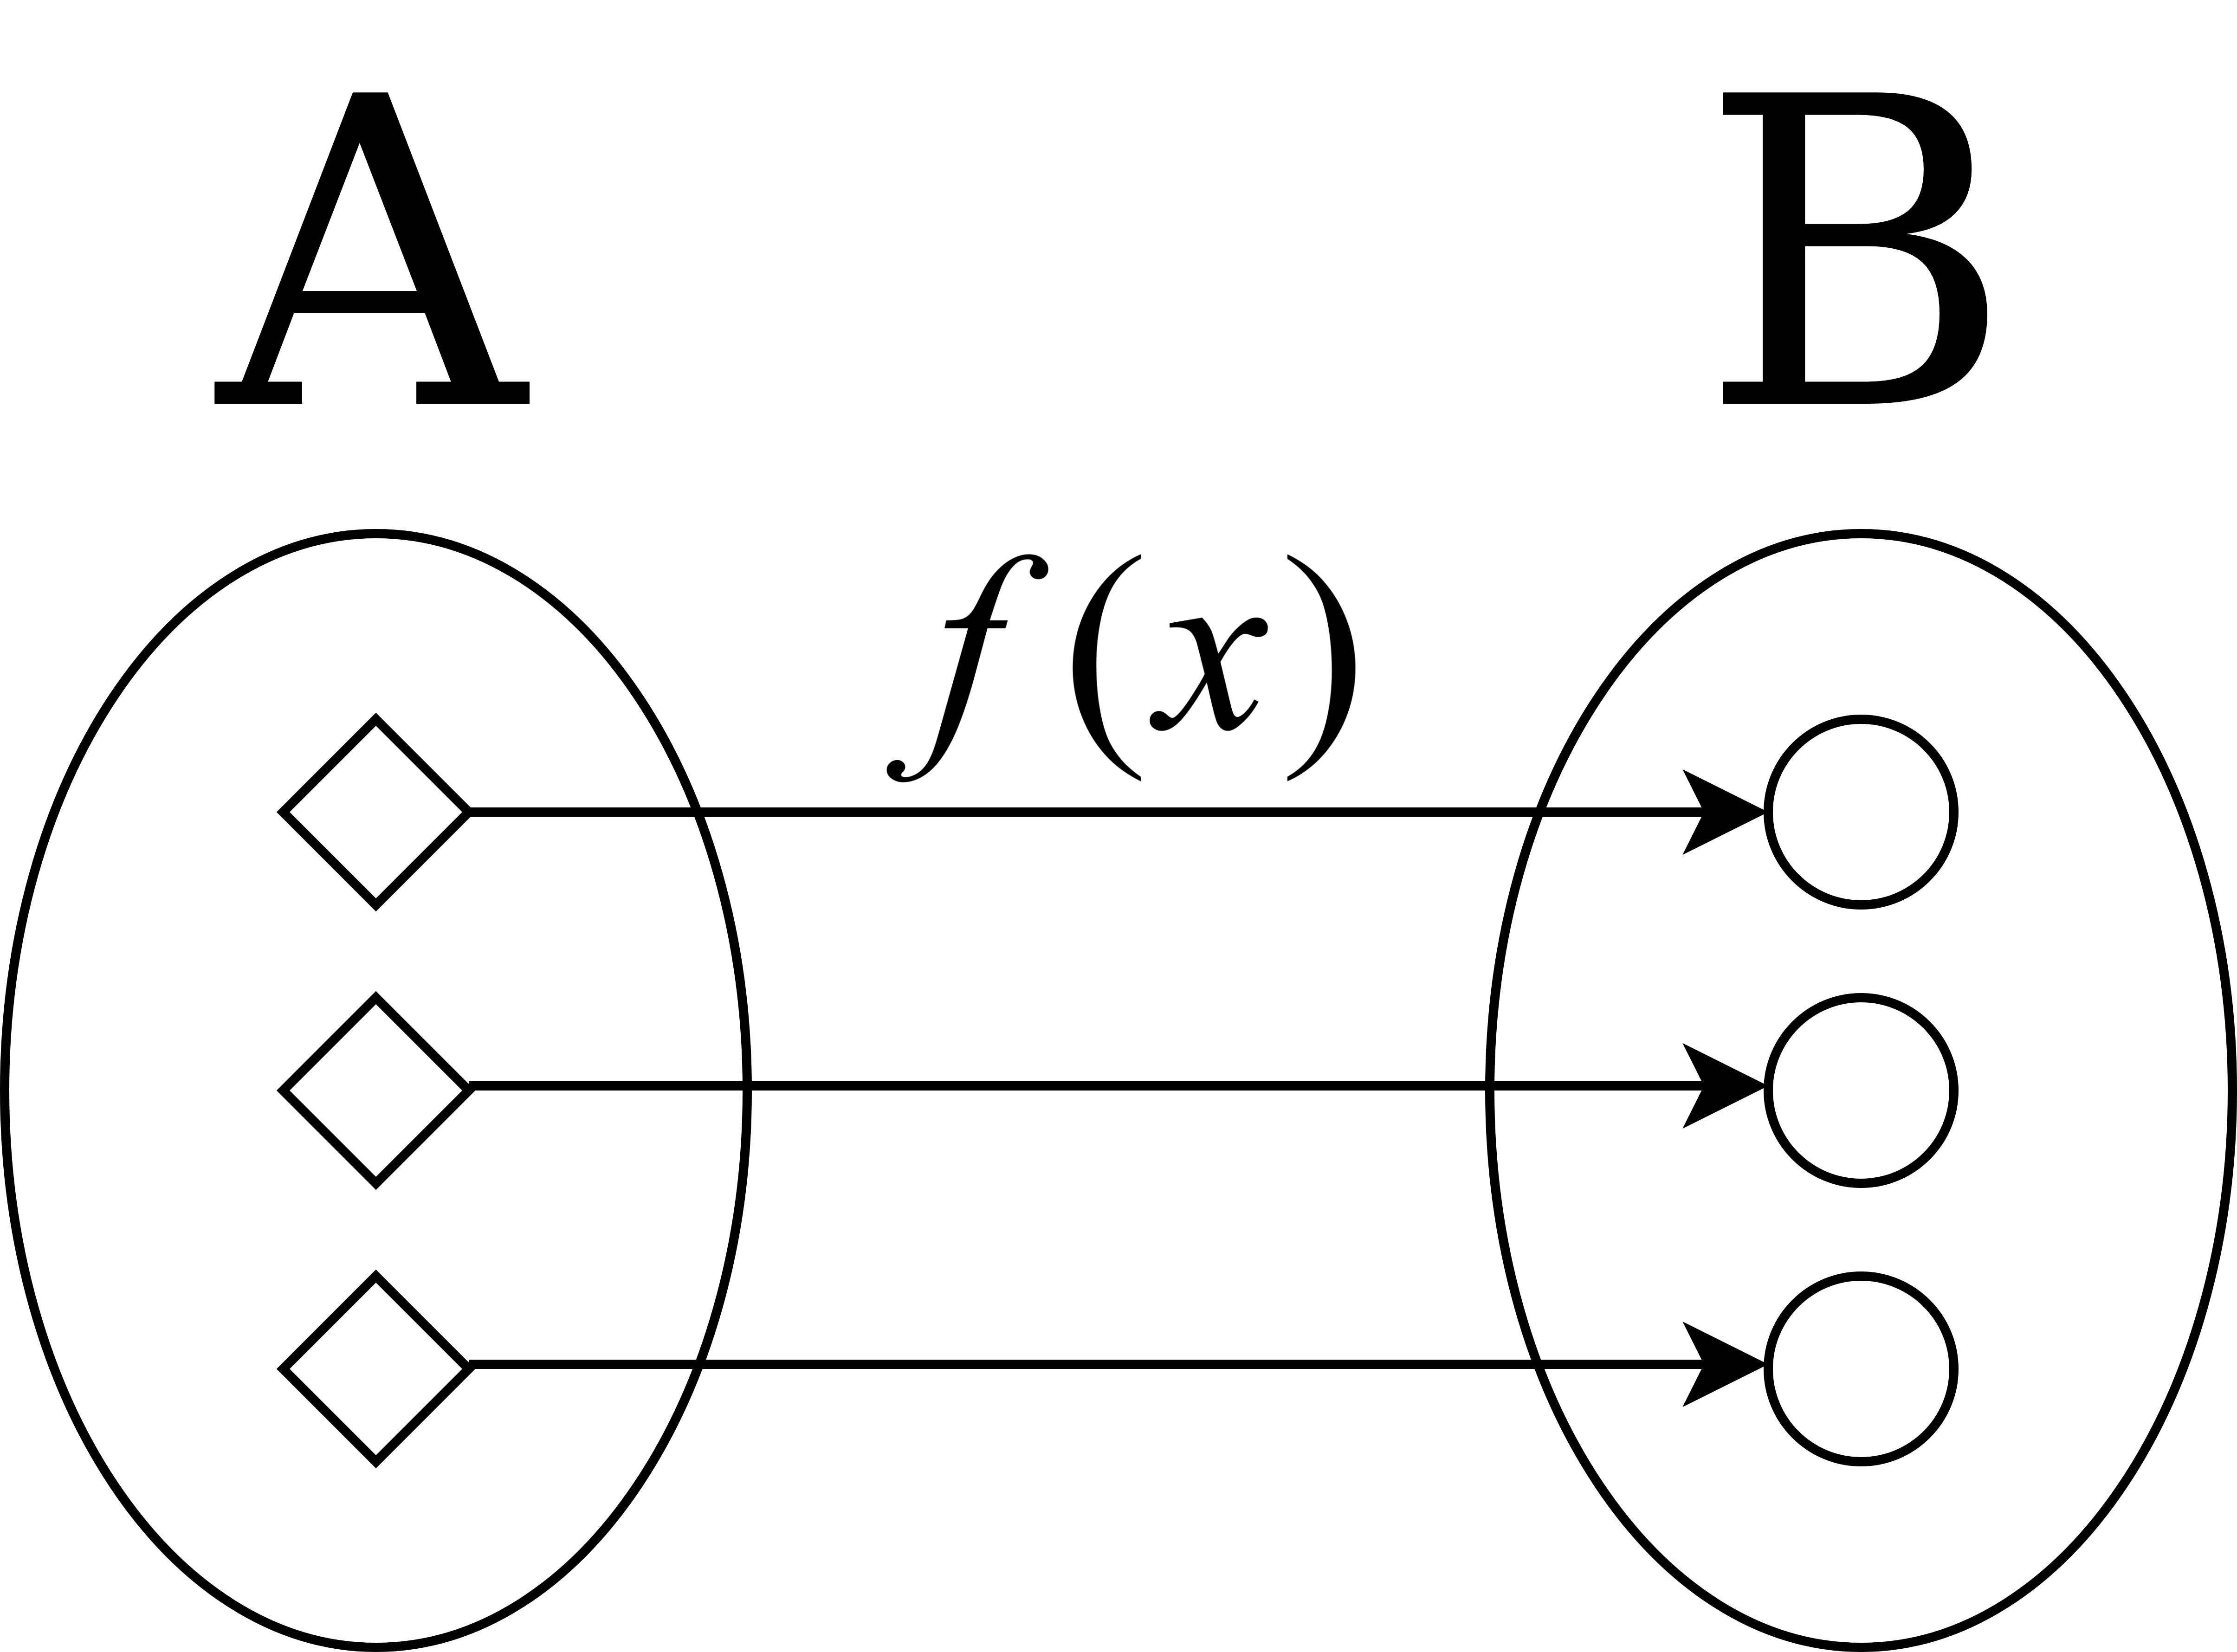
\includegraphics[width=0.5\textwidth]{Function}
  \caption{\label{fig:label} A visual representation of the function f}
\end{figure}


Although this is the mathematical definition, in the domain of programming
languages it could also be stated that "a pure function has no observable effect
on the execution of the program other than to compute a result given its inputs"
\autocite{Chiusano2013FunctionalScala}.

Function constructs in many programming languages don't have the
traits of mathematical functions. One example of it is the one represented in
Listing \ref{lst:addconsole}. This function reads from the console an integer
and returns this read integer added to the parameter n.

\lstinputlisting[
  caption=An example of an impure function,
  captionpos=b,
  label={lst:addconsole}
]{Readline.sc}

This function breaks the definition of a pure function. In figure
\ref{fig:readLineN} a Scala interactive session is ran with the previous
function defined. In this session it can be observed that for the same function input
\texttt{2} two different outputs are returned, \texttt{res1: Int = 5} and \texttt{res1:
  Int = 6} which is a violation of the definition of pure function given before.

\begin{figure}[ht]
  \centering 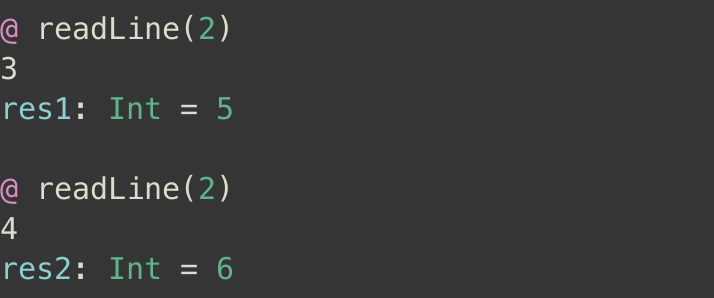
\includegraphics[width=0.5\textwidth]{readline}
  \caption{\label{fig:readLineN} An Scala interactive session showing how the
    \texttt{readLine} function is not pure}
\end{figure}

The elements which make language functions not perform as mathematical functions
are called side effects. To make differentiation functions that don't have side
effects are referred to as pure functions\autocite{UsingAttributes} while
functions that have side effects are called procedures.

Side effects that can make a function not pure are
\autocite{SpulerCompilerEffects}.

\begin{itemize}
  \item Performing I/O
  \item Modifying a variable
  \item Modifying a data structure in place
\end{itemize}

\subsection{Referential transparency} When treating with pure functions there is
a one to one relation between a function call and the result it produces. For
example we can see that the expression $2 + 2$ is the same as $4$. In
mathematics this is a very important property when solving equations. On the
process of solving them usually both sides of it are simplified by applying
operations that reduce the number of elements on each side until we get a simple
expression that its trivial to solve. In figure \ref{fig:refequation} this
process is showcased.

\begin{figure}[ht]
  \centering
  $ 2x - x = \sqrt{16} + 2 \cdot 2$

  $ x = 4 + 4$

  $ x = 8 $
  \caption{\label{fig:refequation} Solving a equation by simplifying with
    referential transparency}
\end{figure}


This property is called referential transparency
\autocite{Strachey2000FundamentalLanguages} and is a very important property of
functional programming.

The reason of why referential transparency is only possible when using pure
functions lies in its definition. If a function is not pure, an element of the
domain may be related with multiple elements of the codomain, thus, it is not
posible to know a priori which is the related element to the input.

\begin{figure}[ht]
  \centering 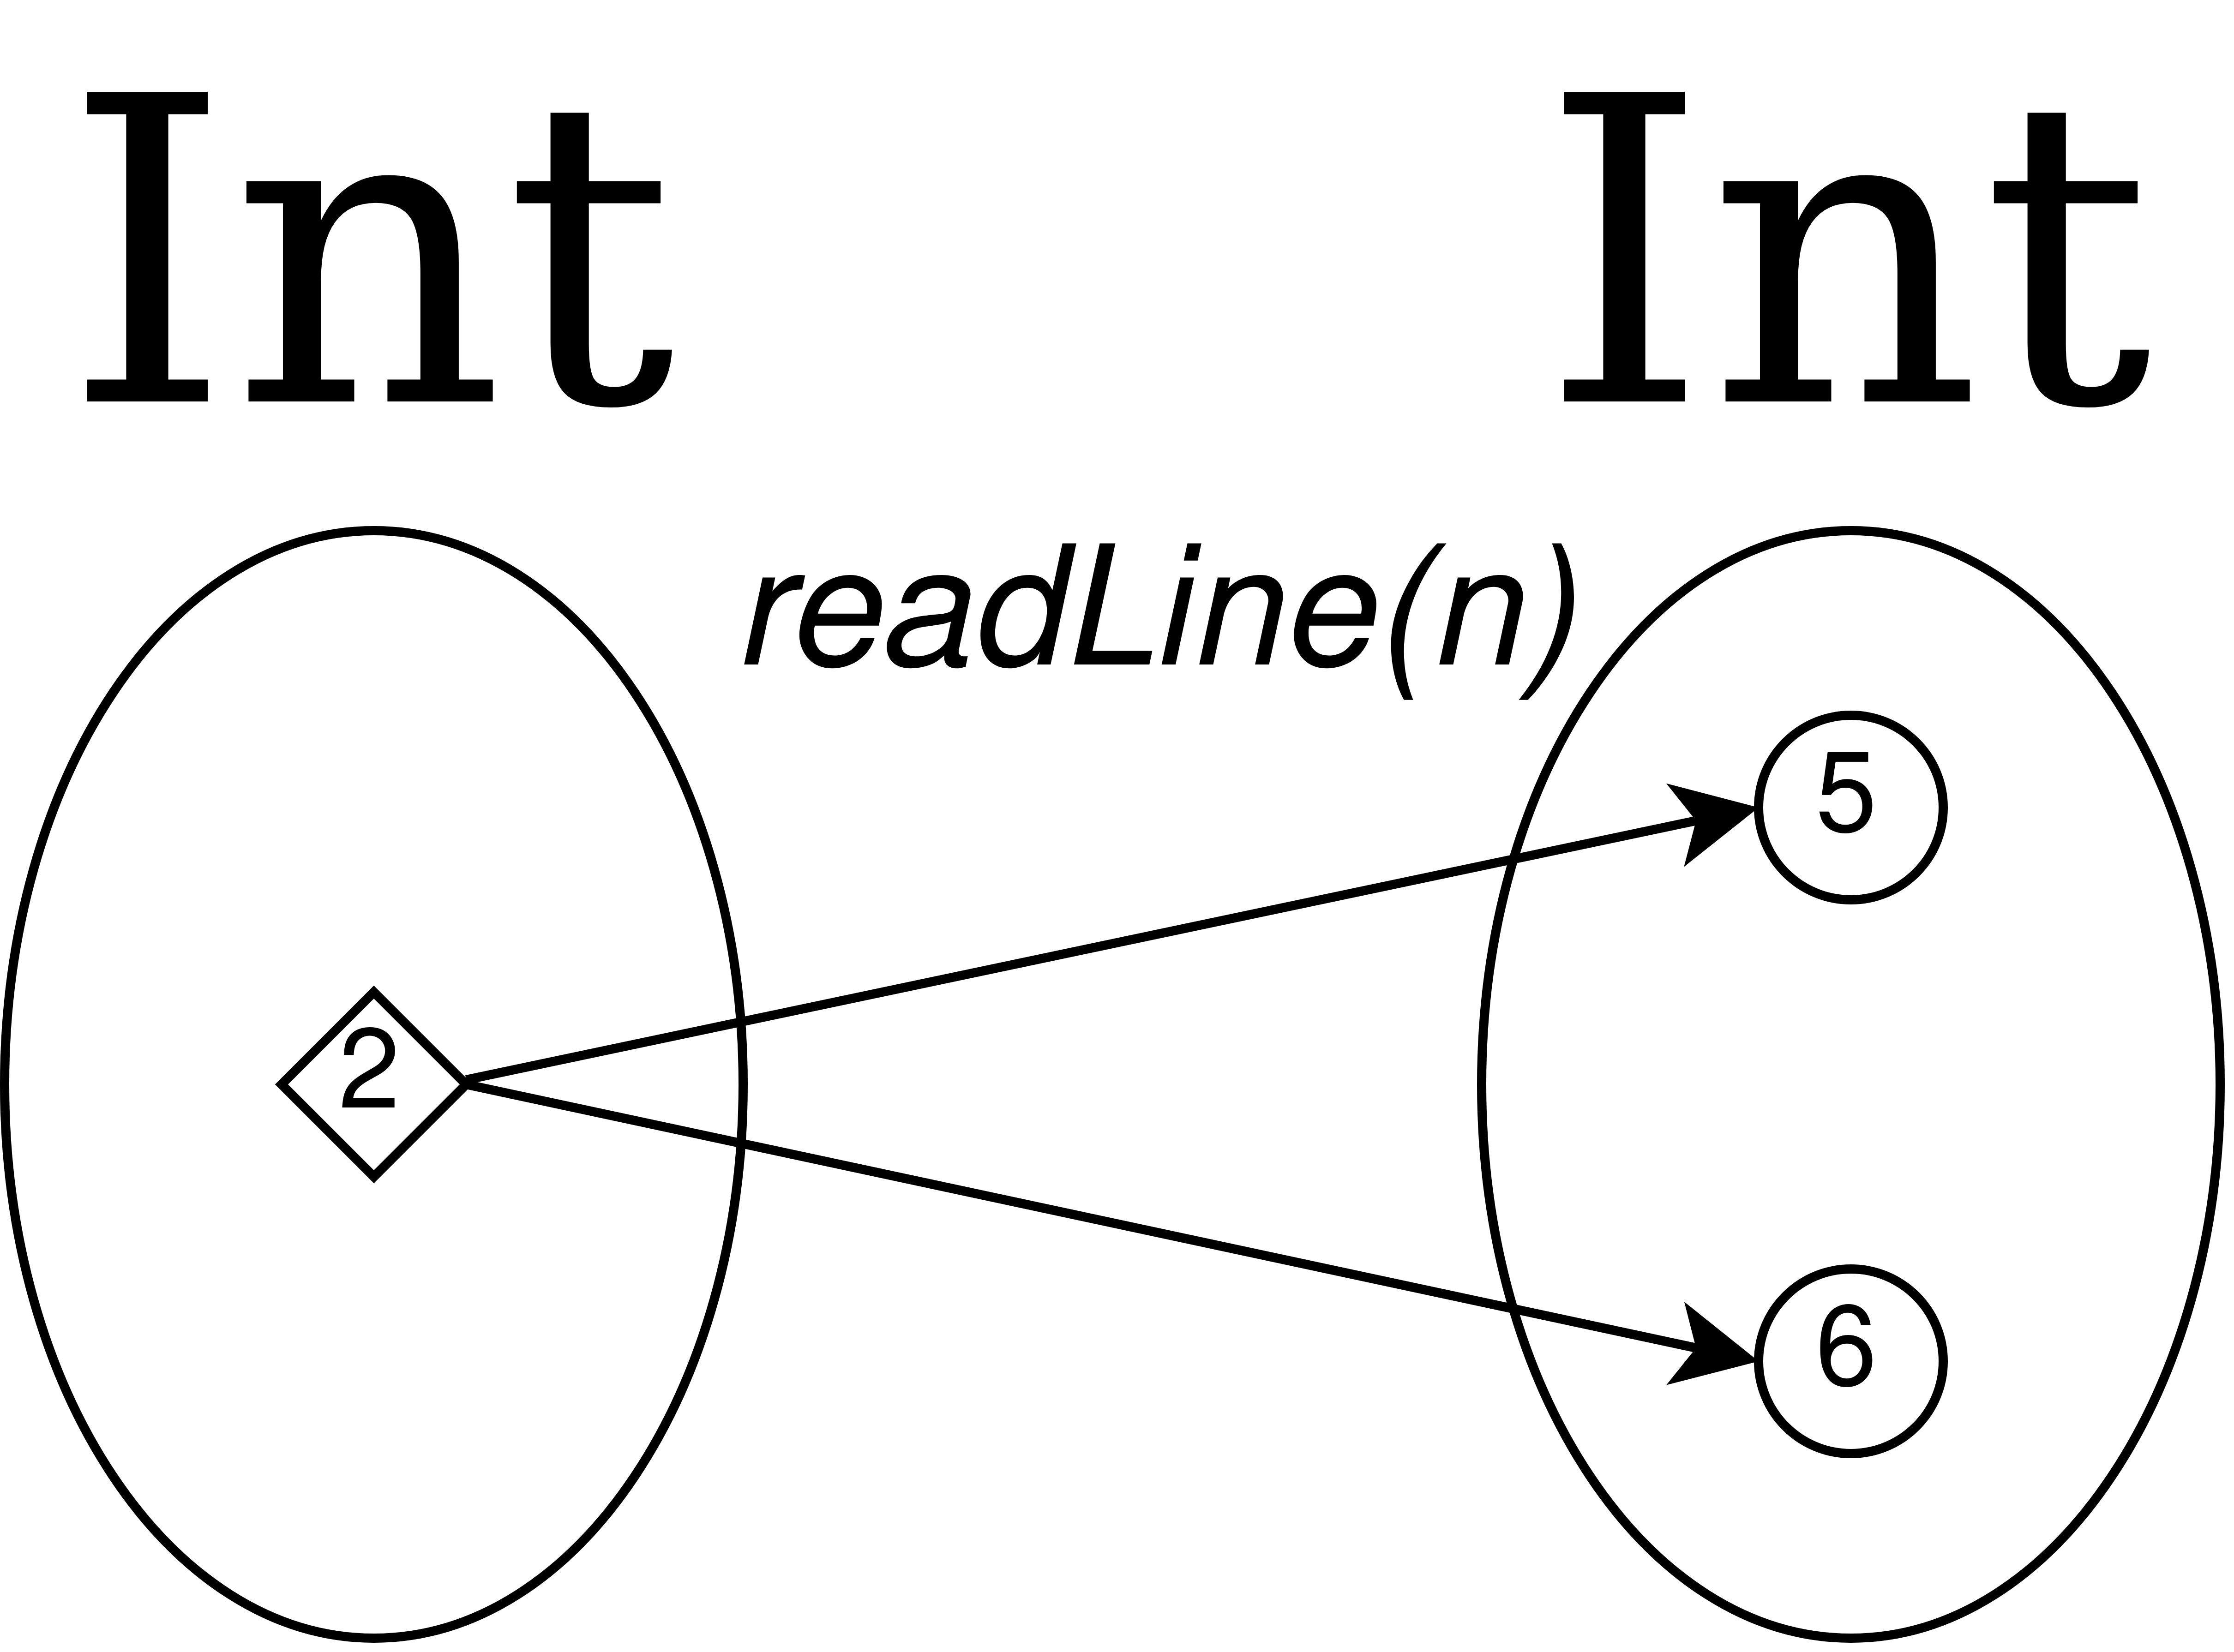
\includegraphics[width=0.5\textwidth]{ImpureFunction}
  \caption{\label{fig:impurefunction} a representation of the relationship of
    the readLine procedure}
\end{figure}

The Figure \ref{fig:impurefunction} represents this indeterminism with the
previously mentioned \texttt{readLine} procedure. The input 2
has two possible results, 5 and 6, and this are not the only possible results.
There are as much as \texttt{Int}s. Which one should be the one substituted? The
given result will only be resolved at run time and thus referential transparency
is lost.

\subsubsection{Local reasoning} One of the benefits of referential transparency
is local reasoning. In order to understand how a function behaves it is only
necesary to understand the components of the function itself and not the context
in which its placed.

When referential transparency is not present this is no longer possible. As an
example consider the function defined in Listing \ref{lst:greeting} which
depends on a global variable \texttt{name}, and returns a greeting to that name.

\lstinputlisting[
  caption=A function which greets \texttt{name},
  captionpos=b,
  label={lst:greeting}
]{Greet.sc}

To understand the behaviour of the function it is needed to know the context in
which it is called, i.e. inspect where the variable \texttt{name} is assigned
and also when assignments to the variable occur previous to the function call.

In the script shown in Listing \ref{lst:greetctx1} it is possible to analyse
that the output Will be \texttt{Greeetings itnaS !} as the name is assigned
to Santi first and then is reversed.

\lstinputlisting[
  caption=An execution of greet which first reverses \texttt{name},
  captionpos=b,
  label={lst:greetctx1}
]{GreetCtx1.sc}

But even though it is possible to analyse the behaviour at a certain point in
time it is not possible to ensure that without changes to the source code of the
function itself the functionality will keep the same. Changes in the context
of the function call regarding the variable \texttt{name} may change the behaviour of
the function in the future. In the script from listing \ref{lst:greetctx2}
without changes to \texttt{greeting} the result of the call is different. In
addition to that the side effect that the \texttt{greetReversed} call made has
been completely overriden.

\lstinputlisting[
  caption=An execution of greet which changes the \texttt{name} after reversing it,
  captionpos=b,
  label={lst:greetctx2}
]{GreetCtx2.sc}

This examples are rather small and thus it is not that difficult to understand
the context, but in an enterprise application where there are many more
components the solution doesn't scale that well. As the uses of the mutable
state increase the understanding of functions which use them start to be more
complex.

\subsubsection{The substitution model and equational reasoning}

When referential transparency is given, a new reasoning model for functional
programs can be achieved, called equational reasoning. When reasoning about a
functional program it is possible to start substituting function calls for the
value they result in. To understand how a program behaves in term of its inputs
the only thing its needed to do is substitute function calls for results they
produce.

This is possible because of the definition of a function. If a function $f$ maps an
element from the domain $a$ to one of the codomain $b$ then $f(a)$ can
transparently be replaced by $b$ and the same kind of substitution that were
presented on the figure \ref{fig:refequation} can be applied to programs.

The substitution model can be useful in multiple scenarios. One example is the
ability to debug errors in a reproducible manner.

The first step is to get the arguments of the misbehaving function. Once they have been acquired the next step is to
start substituting each function call for the value it returns. Whenever the
substitution is made, it is checked that the result of it is the one expected. At the
moment that a function results to a non expected result the cause of the error
is found.

As told before in the local reasoning section this is not possible in a non
functional program, as a function result is not self contained but it depends of
the context in which it is called.

This debugging process can be done automatically by running a debugger which allows to
evaluate expressions on the go. A more manual approach would be by the use of
the use of the Scala REPL (Read–eval–print loop). This tool allows the import
certain functions of a program in a shell which can run them with arbitrary
parameters to help to identify the flaws of programs.

\subsubsection{Function Composition and safe refactoring}

The substitution model can also be used to safely refactor code when repetitions
occur. There are two reasons of why functional code can be safely refactored.
The first is, referential transparency. The second is because of function
composition.

As defined at the beginning of the section functional programs are defined by
the composition of functions. If we have a function \texttt{f: A => B} and
another function \texttt{g: B => C} both can be composed by mathematical
composition $g \circ f$ to create a new function \texttt{h: A => C}. At the
beginning of the section it was stated that this is indeed the essence of
functional programming. Programs are composed by functions that are at the same
times composed of other functions or expressions.

Even programs which define variables which are then used by other functions are
at the end functions defined by composition. This is a corollary of the
substitution model. As variables in functional programming are no more than
named results of expressions, every variable can be substituted by the expression
which produced it. As this expressions can also be composed of other variables
this process has to be done recursively until there are no more variables.

At the very end of the substitutions the only thing that will be left is a pure
expression.

Listing \ref{lst:functionalgreeting} showcases this behaviour. A pure function
like \texttt{greetCapitalized} is no more than the composition of previously defined
functions.

\lstinputlisting[
  caption=An example of how functional programming is about function composition,
  captionpos=b,
  label={lst:functionalgreeting}
]{FunctionalGreeter.sc}

The same function can be defined by the use of intermediate variables instead of
function composition. Listing \ref{lst:variablefunctionalgreeting} is the
transformation of the previous example using intermediate variables. At the end
both functions are semantically equivalent, but the former does explicit
function composition and the other is by the use of intermediate variables.

\lstinputlisting[
  caption=An example of how functional programming is about function composition,
  captionpos=b,
  label={lst:variablefunctionalgreeting}
]{VariableFunctionalGreeter.sc}

Using this principle it is possible to refactor a set of expressions used within
a function to a new one and replace them transparently. This can be achieved
without compromising the programs functionality as long as side effects are not
present in them. If during the program design process it is found repeated code
it can be factored into a function, then substitute the repeated code by the
function call.

\subsection{Functional programming constructs and programming languages} The
functional programming paradigm suits better in some programming languages that
in others. This usually lies in the constructs a language gives to create
programs.

\subsubsection{Statements and expressions} In imperative languages, building
blocks are usually conditional and loop statements. This constructs are
inherently non functional as the way they behave is by having declared variables
that gets updated in this statements. This is very clear in C style for and
while loops.

\subsubsection{Imperative statements} A while loop evaluate an expression. If
this expression is true the block of the while code is executed. In case it is
false the next statement to the block is executed.

The definition of the while loop spots the lack of referential transparency. It
expects that a expression can produce two different values. Some times it will
be false and at least once it will be true if the loop ends.

The for statement have a similar behaviour to the while. With the add of a first
statement that will be executed previous to the first loop and a second one that
will be executed at the end of each loop.

Even if the expression used in the condition of the loops was referential
transparent the statements would add no value to the programs. A condition that
evaluates to true would makes an infinite loop which would never produce any
value and if it was false the block would never get executed.

The if/else statement of imperative languages has the problem that does not
produce any value. The code block of it has to do a side effect, like modifying
a variable, in order to do something useful.

There is one exception in which the if/else statement could produce a value
while not breaking referential transparency. Which is in the case that the
return of the function is done inside the if block. As in Scala this imperative
construct is not present the Listing \ref{lst:functionalifelse} presents this in
the Java class \texttt{FunctionalIf} which showcases in the function
\texttt{abs} how the if construct can be used in a referential transparent manner.

\lstinputlisting[
caption=An example of imperative if else which does not break referential transparency,
captionpos=b,
label={lst:functionalifelse}
]{Java/src/FunctionalIf.java}

\subsubsection{Functional expressions} Functional programming languages by
contrast provide construct that enable composing programs by referential
transparent expressions. To provide conditional logic Scala provides an if/else
expression. In contrast to the if/else statement the expression produces a
value, which is the result of the expression of the block that get executed
\footnote{In case that the if expression doesn't contain an else and the
condition is not satisfied the returned value is the Unit
\autocite{ScalaScala.Unit}}.

Another expression that Scala provides is the for expression. A for expression
traverses a data structure in order to produce a new one by filtering and
transforming the element of it. At a later moment in the document [[Complete
with chapter when ready]] for expressions will be revisited and explained in
greater detail.

Along with the if and the for expressions a way to iterate and construct
functional programs is by using recursion. Recursion is a useful tool in order
to loop through collections without breaking referential transparency. The
problem with recursion is that each nested call makes the run time allocate one
extra frame in the stack to save the context in which the recursive call was
made.

There is a way to overcome this, as functions in which the last expression
calculated is the recursive call, called tail-recursive, can be efficiently
implemented by an optimisation of the compiler which can substitute the
recursive call for a \texttt{goto} statement without the expenses of new stack
frame allocations \autocite{Steele1977DebunkingGoto} \footnote{In Scala in order
to tell the compiler to fail if the substitution cannot be done the
\texttt{@tailrec} annotation can be
used\autocite{ScalaScala.annotation.tailrec}}.

An example can be a function which calculates the sum of a list of integers. To
allow tail recursion a auxiliar function is provided. It accepts an integer
parameter along with the list which accumulates the partial result which is
provided. As the sum operation of integers forms a monoid with 0 as the identity
element the initial call must be made with 0 as Listing \ref{lst:listsum} shows.

\lstinputlisting[
caption=A function summing a list of Integers which doesn't perform a frame
allocation on stack in the recursive call,
captionpos=b,
label={lst:listsum}
]{ListSum.sc}


\subsubsection{Higher order functions} Higher order functions refer to functions
which accept functions as parameters. In Scala functions have their own type,
like \texttt{String}s or \texttt{Int}s do. This way they are treated as other
regular type for the compiler, having the capacity to be passed around as any
other value.

As an example of use of use a string trimming function is shown in listing \ref{lst:stringtrimmer}. This
function will iterate character by character the string and will remove a
character if a specific condition is met. The predicate to remove a character is
decided by the caller. This predicate is a function \texttt{pred: Char => Boolean}

\lstinputlisting[
caption=Trimming a string based on a predicate,
captionpos=b,
label={lst:stringtrimmer}
]{StringTrimmer.sc}

\subsection{Polymorphism in Functional Programming}
\subsubsection{Parametric polymorphism}

One way in which functional programs can express polymorphism by the use of
generic types in function declarations. This mechanism, extended nowadays to
many programming languages, allow functions to take parameters
with an abstract type which will be resolved when the function is called. In Scala to use a generic type in a
function, the generic type
must be defined between square brackets after the function name. This way the
function can be defined one time but be used by different types. The function
filter defined previously for Listing \ref{lst:stringtrimmer} can be generalized
for a generic list \texttt{List[A]} as shown in \ref{lst:listfilter}

\lstinputlisting[
caption=Filtering the elements of a generic List,
captionpos=b,
label={lst:listfilter}
]{Filter.sc}

\subsubsection{Type classes} Although parametric polymorphism is good when the
details of the generic type are irrelevant it lacks the possibility to define a
behaviour that is associated with the type itself.

Type classes \footnote{Not to be confused with classes in Object Oriented Programming} were
defined in Haskell as a way to implement Ad-hoc polymorphism
\autocite{Hall1994TypeHaskell}. A type class is an abstract representation of a
behaviour that types belonging to the class posses. If a type can implement
the type class behaviour it becomes an instance of the type class and it is said
that the type belongs to the class.

In Scala, implicit resolution was implemented as a way to have type classes
resolved at compile time without the need of the function caller to provide the
instance manually and have it resolved automatically by the compiler in an
object oriented language \autocite{Oliveira2010TypeImplicits}.

To illustrate the example a typeclass called \texttt{Show} is presented in
Listing \ref{lst:showtypeclass} with some instances. This typeclass is very
illustrative because in Scala there is a \texttt{toString} method in the
\texttt{Any} class[[Add reference to API]] which every class must extend but it
is very error prone as its default implementation returns the hashCode of the
class, which may not be the wanted implementation. In case that the programmer
forgets to override the method the error can only be caught at run time. When
using the type class if a specific instance is not resolved at compile time the
program will fail to compile improving the overall resilience.

\lstinputlisting[
caption=Different instances of the \texttt{Show} typeclass,
captionpos=b,
label={lst:showtypeclass}
]{Show.sc}

Typeclasses are a very useful form of polymorphism because they allow to decouple structure from
behaviour. If a specific behaviour is desired for a given type it is not needed
to modify the source of the class of it, a type class instance can be provided
in a separate source file. This is specially useful when using third party
libraries. If a new functionality it is required for them as they
are compiled its source code cannot be modified. Nevertheless a type class instance
with the desired functionality can be provided to enrich its capabilities.

There is one way to make the use of typeclasses less cumbersome and more natural
with the use of Implicit Classes. This mechanism allows to wrap an existing
class and add methods which use the instances of the given type class as if they
were of the originally defined for the type.  Listing \ref{lst:typeclasssyntax}
shows how they can be used for our instances.

\subsection{Functional data structures} At the beginning of the section among
the different kind of side effects one of the mentioned was \textit{Modifying a
data structure in place}. If modifying a data structure in place produces a side
effect and breaks referential transparency data structures must be defined
immutable by default, and as a corollary on this property, operations on them
must not modify their internals but return a new one with the changes desired.

Languages that weren't designed to be functional usually define their data
structures as mutable ones. In Java, the Collection class, root of the hierarchy
of a great number of data structures defines most of its operations as mutable
\autocite{Collection}. As an example the method add has the following definition
\texttt{boolean add(E e)}. The returned type of the method is a boolean, which
according to the documentation "is true if this collection changed as a result
of the call". The definition implies that mutation has been done in place.

The main problem with this is that libraries that want to subclass the Java
Collections API and be compatible with the standard library have to maintain
this constraints. This has lead to immutable collection implementations like
Google's Guava Immutable Collection library \autocite{ImmutableCollectionAPI}
serving only as immutable representations of data structures but not providing a
rich set of operations to modify them.

Scala for example provides two type of collections. Immutable and Mutable ones.
Scala documentation states "Scala collections systematically distinguish between
mutable and immutable collections. A mutable collection can be updated or
extended in place. This means you can change, add, or remove elements of a
collection as a side effect. Immutable collections, by contrast, never change.
You have still operations that simulate additions, removals, or updates, but
those operations will in each case return a new collection and leave the old
collection unchanged" \autocite{MutableDocumentation}.
\end{document}